\section{质、量与周延性}

\begin{logicbox}[title=引言]
\textit{标准式直言命题的分析需要掌握其基本特征。本节将详细介绍直言命题的质、量以及词项的周延性,这些概念对于理解命题间的关系和评估推理的有效性至关重要。}
\end{logicbox}

\begin{theorembox}[title=直言命题的质]
\logicterm{质的定义}:每个标准式直言命题或是\logicemph{肯定的}或是\logicemph{否定的},这叫做命题的\logicterm{质}。

\logicemph{肯定命题}:
\begin{itemize}
  \item 如果一个命题肯定了类与类间的包含于关系,不管是全部地还是部分地肯定,那么,它的质就是肯定的
  \item 因此\logicterm{全称肯定命题}(A)和\logicterm{特称肯定命题}(I)的质都是肯定的
  \item 它们的简写名称,即A和I,分别来自于拉丁文"AffIrmo",该词的意思是"我肯定"
\end{itemize}

\logicwarn{否定命题}:
\begin{itemize}
  \item 如果一个命题否定类与类间的包含关系,不管是全部地还是部分地否定,那么,它的质就是否定的
  \item 因此\logicterm{全称否定命题}(E)和\logicterm{特称否定命题}(O)的质都是否定的
  \item 它们的简写名称,即E和O,分别来自于拉丁文"nEgO",该词的意思是"我否定"
\end{itemize}

\logicemph{质的作用}:命题的质决定了谓项的周延性——肯定命题的谓项不周延,否定命题的谓项周延。
\end{theorembox}

\begin{theorembox}[title=直言命题的量]
\logicterm{量的定义}:每个标准式直言命题或是\logicemph{全称的}或是\logicemph{特称的},这称为直言命题的\logicterm{量}。

\logicemph{全称命题}:
\begin{itemize}
  \item 如果一个命题述及主项所指称的类的所有元素,那么,它的量就是全称的
  \item 因此\logicterm{A命题}和\logicterm{E命题}的量都是全称的
  \item 全称命题的主项总是周延的
\end{itemize}

\logicwarn{特称命题}:
\begin{itemize}
  \item 如果一个命题只述及主项所指称的类的某些元素,那么,它的量就是特称的
  \item 因此\logicterm{I命题}和\logicterm{O命题}的量都是特称的
  \item 特称命题的主项总是不周延的
\end{itemize}

\logicemph{量词标识}:
\begin{itemize}
  \item 每个标准式直言命题都以"\textbf{所有}"、"\textbf{没有}"或者"\textbf{有}"等词开头,这些词表明了命题的量
  \item "所有"和"没有"表示命题是全称的
  \item "有"表示命题是特称的
  \item 另外,"没有"还表明了E命题的质是否定的
\end{itemize}

\logicwarn{命名规律}:我们发现"全称肯定"、"全称否定"、"特称肯定"和"特称否定"这几个名称都是先描述量再描述质,从而唯一地描述了每一种标准式直言命题。
\end{theorembox}

\subsection{标准式直言命题的一般模式}
每个标准式直言命题的主项、谓项之间都有一个动词形式"\textbf{是}"(O命题需在"是"前面加上一个"不"字),这个动词把主项和谓项联结起来,称为\textbf{联项}(copula)。前一节给出的公式中的联项只有"是"和"不是"两种,但依据不同的措辞需要,有时可能用其他形式的联项更为适当。例如,下面三个命题中:

\begin{quote}
有罗马统治者曾经是(were)独裁者。\\
所有正方形均为(are)四边形。\\
有士兵不会成为(will not be)英雄。
\end{quote}

联项分别是"曾经是"、"均为"和"不会成为"。标准式直言命题的一般模式由四个部分组成:首先是\textbf{量项},其次是\textbf{主项},再次是\textbf{联项},最后是\textbf{谓项}。可以记为:

量项(主项)联项(谓项)。

\begin{theorembox}[title=周延性的基本概念]
\logicemph{基础理解}:基于类的解释,标准式直言命题指称的都是对象的类,而命题被看做是关于这些类的。当然,命题谈及类的方式不尽相同。

\logicwarn{谈及方式}:一个命题可能谈及一个类的全部元素,也可能只谈及这个类的一些元素。

\logicemph{典型例子}:下面这个命题:

\begin{quote}
所有参议员是公民。
\end{quote}

\logicwarn{分析结果}:
\begin{itemize}
  \item 述及或曰关乎全部参议员,但没有述及所有公民
  \item 它断定的是参议员类的任何一个元素都是公民
  \item 但并没有就所有公民做出断言
  \item 它既没有肯定,也没有否定所有公民都是参议员
\end{itemize}

\logicemph{一般规律}:任何一个有如下形式的A命题:

\begin{center}
所有$S$是$P$。
\end{center}

都述及了主项$S$指称的类的全部元素,但并没有述及谓项$P$指称的类的全部元素。

\logicterm{周延性定义}:我们引入"\logicterm{周延}"这个技术性术语,用以刻画出现于直言命题中的主谓项的性质。如果一个命题述及了某个词项所指称的类的全部元素,则称该词项在这个命题中是\logicterm{周延的}。

\logicwarn{分析目标}:我们来考察一下各种标准式直言命题,看看其中哪些词项周延、哪些词项不周延。
\end{theorembox}

\begin{examplebox}[title=各类命题的周延性分析]
\logicemph{A命题的周延性}:
\begin{itemize}
  \item \logicwarn{例子}:仍以"所有参议员都是公民"为例
  \item \logicterm{主项}:A命题的主项(在命题中)是\textbf{周延的}
  \item \logicterm{谓项}:而谓项(在命题中)是\textbf{不周延的}
  \item \logicemph{原因}:命题述及了主项指称类的全部元素,但没有述及谓项指称类的全部元素
\end{itemize}

\logicwarn{E命题的周延性}:
\begin{itemize}
  \item \logicwarn{例子}:接下来看E命题,比如:"没有运动员是素食主义者。"
  \item \logicemph{逻辑分析}:这样的E命题,断定了任何一个运动员都不是素食主义者。整个运动员的类都被排除在素食主义者的类之外
  \item \logicterm{主项周延}:由于E命题述及了主项指称的类的全部元素,因此可以说E命题的主项是周延的
  \item \logicterm{谓项周延}:由于断定了整个运动员的类被排除在素食主义者的类之外,这个命题也就断定了整个素食主义者的类也被排除在整个运动员的类之外
  \item \logicwarn{结论}:E命题的主项周延,谓项也周延
\end{itemize}

\logicemph{I命题的周延性}:
\begin{itemize}
  \item \logicwarn{例子}:说到I命题,情况就有所不同了。例如:"有士兵是胆小鬼。"
  \item \logicemph{特点}:既没有对所有士兵进行断定,也没有对所有胆小鬼进行断定
  \item \logicterm{关系性质}:不能说一个类完全包含于另一个类之中,也不能说完全排除在外
  \item \logicwarn{结论}:在任何特称肯定命题中,主项、谓项都是\textbf{不周延的}
\end{itemize}

\logicwarn{O命题的周延性}:
\begin{itemize}
  \item \logicwarn{例子}:特称否定命题或者说O命题,例如:"有些马不是良种马。"
  \item \logicterm{主项}:与特称肯定命题一样,主项不周延。并不言说所有的马,而只述及主项指称的类的一些元素
  \item \logicemph{谓项分析}:它说的是所有马中被排除在良种马之外的那一部分,亦即这部分被排除在后一个类的全体之外
  \item \logicterm{谓项周延}:说某事物被排除在一个类之外,也就述及了这个类的全部。正像说一个人被排除在某个国家之外,就等于说这个国家的任何地方都不接纳此人一样
  \item \logicwarn{结论}:特称否定命题的谓项是\textbf{周延的},但主项\textbf{不周延}
\end{itemize}
\end{examplebox}

\begin{theorembox}[title=周延性规律总结]
\logicemph{基本规律}:周延性问题可以总结如下:

\logicwarn{主项的周延性}(由量决定):
\begin{itemize}
  \item \logicterm{全称命题},包括肯定的和否定的,其主项是周延的
  \item \logicterm{特称命题},不管是肯定的还是否定的,其主项都是不周延的
  \item 也就是说,标准式直言命题的\textbf{量决定了主项的周延情况}
\end{itemize}

\logicemph{谓项的周延性}(由质决定):
\begin{itemize}
  \item \logicterm{肯定命题},无论全称的还是特称的,其谓项都是不周延的
  \item \logicterm{否定命题},包括全称的和特称的,其谓项都是周延的
  \item 也就是说,标准式直言命题的\textbf{质决定了谓项的周延情况}
\end{itemize}

\logicwarn{四种命题的周延性模式}:
\begin{itemize}
  \item \logicterm{A命题}:主项周延,谓项不周延
  \item \logicterm{E命题}:主项周延,谓项周延
  \item \logicterm{I命题}:主项不周延,谓项不周延
  \item \logicterm{O命题}:主项不周延,谓项周延
\end{itemize}

\logicemph{记忆口诀}:
\begin{itemize}
  \item 量决定主项:全称周延,特称不周延
  \item 质决定谓项:肯定不周延,否定周延
\end{itemize}
\end{theorembox}

\begin{center}
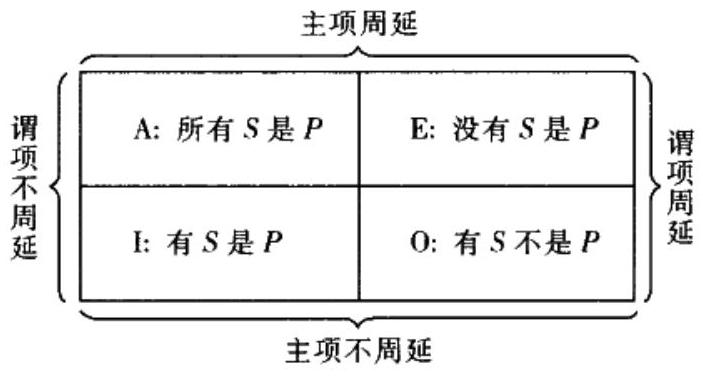
\includegraphics[width=\textwidth]{images/2025_05_15_6a28331d5e7c993ad07ag-234.jpg}

图 5-2 周延性总结
\end{center}

\chaptersummary{
直言命题的\logicterm{质}(肯定或否定)决定谓项的周延性,\logicterm{量}(全称或特称)决定主项的周延性。\logicterm{周延性}指命题述及词项所指称类的全部元素。四种标准式命题的周延性规律:A命题主项周延谓项不周延,E命题主谓项都周延,I命题主谓项都不周延,O命题主项不周延谓项周延。
}